% !TeX spellcheck = en_US
\documentclass[a4paper, 10pt]{article}
\usepackage[utf8]{inputenc}
\usepackage[inline]{enumitem}
\usepackage{amsmath, graphicx, subcaption, xcolor}

\title{Some Title}
\author{Authors}
\date{\today}

%%%% Local definitions %%%%
\newcommand{\bubblecoach}{\ensuremath{\mathcal{C}_{\rm bubble}}}
\newcommand{\quickcoach}{\ensuremath{\mathcal{C}_{\rm quick}}}
%%%%%%%%%%%%%%%%%%%%%%%%%%%

%%%% Editor's commands %%%%
\newcommand{\edcom}[1]{{\sf\color{red}$>>>$ #1}}
\newcommand{\tbc}{\edcom{To be completed\ldots}}
\newcommand{\ednote}[1]{\marginpar{\flushleft\tiny\sf\color{red}{#1}}}
%%%%%%%%%%%%%%%%%%%%%%%%%%%

\begin{document}
	%
	\maketitle
	%
	\section{Introduction}\label{sec:introduction}
	%
	\tbc
	%
	%
	%
	\section{Related Literature}\label{sec:related-literature}
	%
	\tbc
	%
	%
	%
	\section{Experimental Setup}\label{sec:experimental-setup}
	%
	In this Section we empirically explore coachable searching as an approach to preference elicitation, by having a machine learner iteratively seek advice by a proxy coach, as in \cite{}, with the aim of iteratively improving its search capacity, as per the coach's explicit or implicit search policy. Two experimental procedures, one aiming to assess the efficacy and scalability of the coaching process and one to explore a more realistic and open--ended environment.\ednote{Add a few words about how coaching happens in the context of searching, i.e., how from a past sub--optimal state the coach provides a piece of advice according to their (implicit / explicit) policy that improves the state towards a(n implicit / explicit) goal.}
	%
	%
	%
	\subsection{Sorting Coaching}\label{subsec:sorting-coaching}
	%
	In this series of coaching sessions we have implemented two variants of a machine coach, aiming to explain to an initial ignorant agent about how to sort a list of numbers, as a rough equivalent to linear preference elicitation. The first coach, \bubblecoach, uses bubble sort as its underlying policy while the second one, \quickcoach, uses quicksort to provide advice from. We explored different state sizes, $n$, ranging from $1$ to $20$, running $m=100$ iterations for each value of $n$. We have also explored two different types of advice for each coach:
	\begin{enumerate*}[label=(A\arabic*)]
		\item \emph{full advice}, where each piece of advice depends on the entire state, and;
		\item \emph{partial advice}, where each piece of advice depends on the specific part of the state to be improved.
	\end{enumerate*}
	Moreover, for each advice type we have considered three learner configurations regarding advice memory:
	\begin{enumerate*}[label=(C\arabic*)]
		\item \emph{no memory} across different iterations for the same state size, $n$, i.e., coaching sessions are pairwise independent;
		\item \emph{short memory} across different iterations for the same state size, $n$, i.e., coaching sessions across different values of $n$ are independent but not within the same value for $n$, and;
		\item \emph{long memory} across all values of state size, $n$, so all coaching sessions are correlated, building on knowledge from previous test cases.
	\end{enumerate*}
	In Figures~\ref{fig:full and partial sorting coaching results}.
	
	\begin{figure}[!tb]
		\centering%
		\hfill%
		\begin{subfigure}[t]{0.47\textwidth}
			\centering
			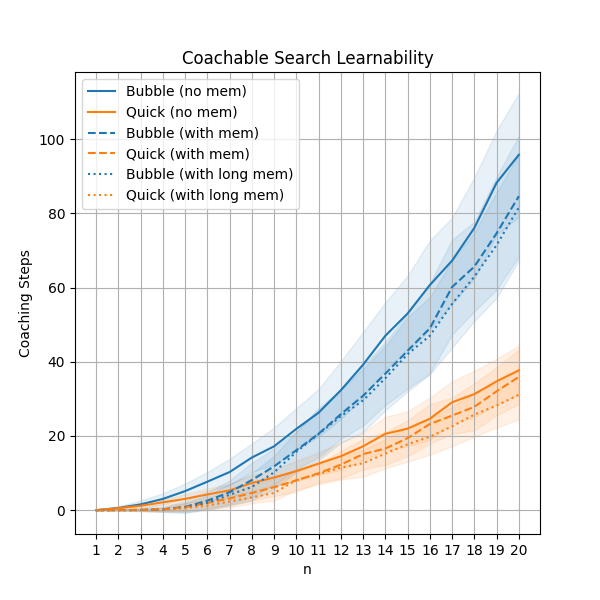
\includegraphics[width=\linewidth]{../CLARIF-i-stable/plots/full_condition_learnability.png}
			\caption{\tbc}
			\label{fig:full sorting coaching results}
		\end{subfigure}%
		\hfill%
		\begin{subfigure}[t]{0.47\textwidth}
			\centering
			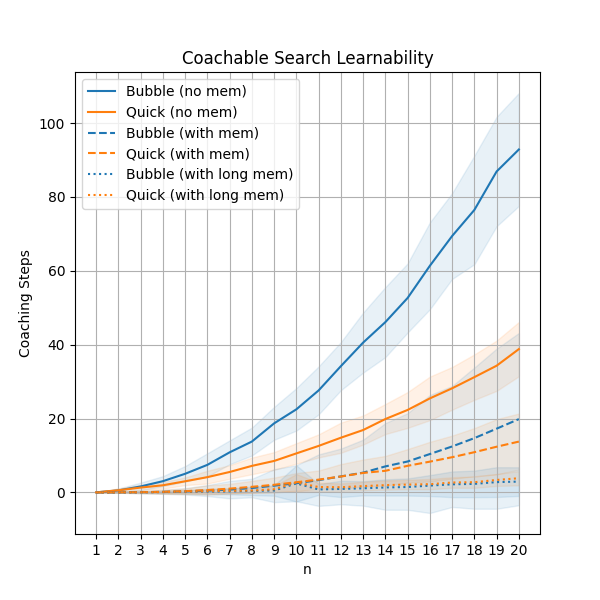
\includegraphics[width=\linewidth]{../CLARIF-i-stable/plots/partial_condition_learnability.png}
			\caption{\tbc}
			\label{fig:partial sorting coaching results}
		\end{subfigure}%
		\hfill%
		\caption{\tbc}
		\label{fig:full and partial sorting coaching results}
	\end{figure}
	%
	%
	%
	\section{Results}\label{sec:results}
	%
	\tbc
	%
	%
	%
	\section{Conclusions and Future Work}\label{sec:conclusions-and-future-work}
	%
	\tbc
	%
	%
	%
\end{document}
